\documentclass{article}
% --- watermark (auto-inserted) ---
\usepackage{xcolor}
\usepackage{xfp}% \fpeval; in the kernel since 2022, harmless on older LaTeX
\usepackage{draftwatermark}
\newlength{\watermarkTextWidth}
\AddToHook{begindocument/end}{%
  \SetWatermarkText{\normalfont Generated by The Agentic Scientist}%
  \SetWatermarkFontSize{10pt}%
  \SetWatermarkLightness{0.85}%
  \settowidth{\watermarkTextWidth}{\normalfont\fontsize{10pt}{12pt}\selectfont Generated by The Agentic Scientist}%
  \edef\watermarkScale{\fpeval{0.8 * sqrt(\paperwidth**2 + \paperheight**2) / \watermarkTextWidth}}%
  \edef\watermarkAngle{\fpeval{atand(\paperheight/\paperwidth)}}%
  \SetWatermarkScale{\watermarkScale}%
  \SetWatermarkAngle{\watermarkAngle}%
}
% --- end watermark ---

\usepackage{iclr2026_conference,times}
\usepackage{amsmath,amssymb,booktabs,graphicx,subcaption}
\usepackage{hyperref,url}
\title{Variance-Guided Benchmark Selection for\newline Incomplete Model Score Matrices}
\author{}

\begin{document}
\maketitle

\begin{abstract}
Historical leaderboard scores offer a way to reduce model evaluation costs: measure a small subset of benchmarks and predict the rest. No improvement beyond the original reference was established; we characterize its variance-guided masked low-rank policy. Historical scores determine benchmark factors; purchased scores determine a new model's latent representation; a conditional variance proxy determines which benchmark to purchase. The selector depends on availability and previous query identities, not observed score values. On separately fitted MTEB embedding-model and Open LLM generative-model matrices, using model-disjoint and heuristic name-family-disjoint splits, the pooled normalized prediction score is $0.9528$, versus $0.9364$ for random-query low-rank reconstruction. The supplied paired family-clustered interval for this difference is $[0.0148,0.0185]$. Independently deranging historical columns reduces the studied score to $0.9234$, consistent with useful cross-benchmark correspondence. However, information-selected covariance ridge is competitive, and different query policies leave different evaluation targets. The evidence therefore supports a conditional comparison of complete evaluation policies, not fixed-target superiority, response-adaptive acquisition, or a universal sufficient benchmark budget.
% @evidence[[paper_data.json#final_evaluation.metrics]]
% @evidence[[paper_data.json#downstream_study]]
\end{abstract}

\section{Introduction}
Evaluating a new language model across a broad benchmark suite is costly even when each individual benchmark is inexpensive. Public leaderboards contain a different resource: repeated measurements of historical models on overlapping tasks. If these measurements share structure, a small number of newly purchased benchmark scores may help estimate the unmeasured scores. The practical question is not just whether benchmarks correlate, but whether an explicit selection-and-prediction policy uses a limited evaluation budget more effectively than simpler alternatives.

We consider an incomplete matrix whose rows are models and columns are benchmark measurements. A new row comes with an availability mask indicating which measurements could be obtained. The policy purchases a bounded number of entries and predicts the available entries that remain unpurchased. This formulation separates historical missingness from the new model's query budget. It also exposes a subtle evaluation issue: selecting a benchmark removes that benchmark from the scored remainder. Two selection policies may therefore be evaluated on different target sets even when they start from the same model and availability mask.

Our central hypothesis is deliberately limited: \emph{a variance-guided query rule coupled to masked low-rank reconstruction provides a useful operational policy when historical cross-benchmark correspondence is informative}. The method is an inspectable combination of regularized matrix factorization and prediction-oriented design, rather than a new architecture. We compare it with a matched factor predictor using random queries, two covariance-ridge policies, historical benchmark means, and an observation-using mean-offset predictor. The matrices are fitted independently; transferring a protocol across embedding and generative models is not transferring learned factors between them.

The final evaluation supports this hypothesis within the measured regime. The studied policy has the highest pooled score among the six evaluated policies, with a positive paired uncertainty interval against random-query factor reconstruction. Destroying historical row correspondence across columns lowers its score. Neither result identifies a universally optimal selector: covariance ridge nearly matches the pooled result and slightly exceeds it in one retained source/split/seed cell. Moreover, the variance proxy optimizes a working squared-error quantity, whereas the measured loss is absolute error on a changing remainder.
% @evidence[[paper_data.json#final_evaluation.metrics]]
% @evidence[[paper_data.json#final_evaluation.evaluation_evidence.episodes]]

The contributions are threefold. First, we specify a reproducible, CPU-only policy connecting incomplete historical scores to budgeted reconstruction. Second, we provide a direct comparison across two distinct public leaderboard sources, with row-level and name-family-level separation and paired uncertainty for the closest selector comparison. Third, we use a historical-correspondence control and explicitly separate what these measurements establish from what requires fixed-target, family-aware, or score-adaptive experiments. The contribution is this bounded empirical characterization, not evidence that unmeasured alternatives underperform.

\begin{figure}[t]
\centering

\includegraphics[width=\textwidth]{figures/concept_overview.png}
\caption{Budgeted reconstruction from historical benchmark scores. Each source is fitted separately. Masked historical measurements yield benchmark factors; a variance proxy chooses an available benchmark; purchased scores determine a latent representation used to predict the unpurchased remainder. The query rule does not condition on purchased values. The evaluated remainder changes with the query policy.}
\label{fig:overview}
\end{figure}

\section{Related Work}
\paragraph{Evaluation breadth and compression.}
MMLU, MTEB, and HELM illustrate the breadth and heterogeneity of model evaluation \citep{MMLU,MTEB,HELM}. Their roles differ: MTEB evaluates embeddings, whereas the other settings concern language-model capabilities more broadly. Reducing evaluation within a benchmark, as in tinyBenchmarks \citep{Tiny}, is distinct from purchasing complete benchmark scores. Metabench uses sparse item-level measurements to estimate underlying benchmark abilities \citep{Metabench}; our observational unit is instead an already aggregated model--benchmark score. BenchBench emphasizes that agreement conclusions depend on evaluation choices \citep{BenchBench}. We accordingly state the precise prediction target rather than treating correlation or a high aggregate score as sufficient validation.

\paragraph{Latent structure and experimental design.}
Observational scaling laws and Sloth motivate low-dimensional descriptions of multi-benchmark performance \citep{Observational,Sloth}. We do not fit compute scaling laws or recover interpretable skills. Our factors are regularized predictive coordinates, following the broader matrix-factorization tradition \citep{Koren,PMF,BayesianMF}. Masked numerical ratings should not be confused with implicit positive/negative feedback \citep{Hu}. Matrix completion has both convex and alternating-minimization approaches \citep{CandesRecht,CandesTao,Keshavan,Mazumder,Jain}; their recovery guarantees require assumptions not verified for these selectively observed leaderboards. Ridge regularization stabilizes the conditional solves \citep{Hoerl}. The acquisition rule is a prediction-oriented design heuristic, related to Bayesian design and statistical active learning \citep{Chaloner,Cohn}, not a theorem of absolute-error optimality.

\paragraph{Missingness and uncertainty.}
Classical missing-data work distinguishes the observed-data model from assumptions about the observation process \citep{Rubin,Schafer}. Optimizing a masked loss does not establish that missing leaderboard entries are ignorable, nor is our alternating ridge fit a fitted model of that process or an EM analysis \citep{Dempster}. Bootstrap inference also depends on the resampling unit \citep{Efron}. Work on dependent data arrays cautions against treating all cells as independent \citep{Owen}. Here the supplied interval resamples heuristic families in a paired fashion; it does not quantify every source of distributional or implementation uncertainty.

\section{Method}
\label{sec:method}
\subsection{Problem and success criterion}
Let $X\in[0,1]^{M\times N}$ be historical scores, with observed-entry mask $W$. For a held-out model, let $A$ denote the available benchmark indices, $Q_k\subset A$ the purchased indices after budget $k$, and $x_j$ the measured score at index $j$. The predictor receives only $X,W,A$, and purchased values. It outputs $\hat x_j$ for the remaining targets $R_k=A\setminus Q_k$. For one held-out row, the reported normalized prediction score is
\begin{equation}
 S_k=1-\frac{1}{|R_k|}\sum_{j\in R_k}
 \left|\operatorname{clip}_{[0,1]}(\hat x_j)-x_j\right|.
 \label{eq:score}
\end{equation}
% @evidence[[source_evidence/evaluation/evaluate_final.py#curve_score]]
Higher is better. This is not classification accuracy, explained variance, or a fraction of recovered benchmarks. Each benchmark purchase has equal nominal cost; the objective does not incorporate measured benchmark runtimes. Missing historical cells contribute no observations, even though the transport representation stores zeros in those positions. The new model's availability mask is supplied before selection, which is more information than an evaluator may have in a prospective deployment.

\subsection{Masked factors and conditional prediction}
For benchmark $j$, compute the historical observed mean $\mu_j$. With latent row coordinates $u_i\in\mathbb R^r$ and benchmark factors $v_j\in\mathbb R^r$, the fitted objective is
\begin{equation}
 \min_{U,V}\sum_{i,j:W_{ij}=1}(X_{ij}-\mu_j-u_i^\top v_j)^2
       +\lambda\left(\|U\|_F^2+\|V\|_F^2\right).
 \label{eq:fit}
\end{equation}
The means remain fixed during alternating ridge updates. Initialization uses the leading right singular vectors of the zero-filled, mean-centered matrix, scaled by square roots of their singular values. Zero filling is an initialization device, not a claim that missing measurements equal a benchmark mean in the fitted loss.

The regularization coefficient is $\lambda=0.1$. Rank is chosen from $\{1,2,4,8\}$ by absolute error on a deterministic seeded holdout of approximately $10\%$ of observed historical cells. Infeasible ranks are skipped. Each rank uses at most four alternating sweeps for validation; the chosen rank is refitted on all historical observations for at most eight sweeps, capped by the requested fitting allowance. This is historical-cell validation, not nested validation on held-out model families. The saved results do not report selected ranks, so we do not attribute performance to a particular latent dimensionality.
% @evidence[[source_evidence/downstream/program/src/program.py#L45-L83]]

For a new model and purchased set $Q$, stack the corresponding factor rows into $V_Q$. Prediction uses
\begin{equation}
 C_Q=(V_Q^\top V_Q+\lambda I)^{-1},\qquad
 \hat u_Q=C_QV_Q^\top(x_Q-\mu_Q),\qquad
 \hat x_j=\operatorname{clip}_{[0,1]}(\mu_j+v_j^\top\hat u_Q).
 \label{eq:predict}
\end{equation}
Each new model has an independent conditional state. Observations from one held-out row do not update another row's latent representation or refit the historical benchmark factors.
% @evidence[[source_evidence/downstream/program/src/program.py#L110-L142]]

\subsection{Variance-guided benchmark acquisition}
Let $T=A\setminus Q$ be the currently available, unpurchased indices. For each legal next query $a\in T$, the implemented proxy is
\begin{equation}
 g(a\mid Q,A)=\frac{\sum_{j\in T}(v_j^\top C_Qv_a)^2}
                         {1+v_a^\top C_Qv_a},\qquad
 a^*=\arg\max_{a\in T}g(a\mid Q,A).
 \label{eq:acq}
\end{equation}
% @evidence[[source_evidence/downstream/program/src/program.py#L114-L127]]
The index order resolves ties. Under a unit-noise linear working model, adding $v_a$ changes the inverse information matrix by
\begin{equation}
 C_{Q\cup\{a\}}=C_Q-
 \frac{C_Qv_av_a^\top C_Q}{1+v_a^\top C_Qv_a}.
 \label{eq:rankone}
\end{equation}
Consequently, $g$ is the reduction in $\operatorname{tr}(V_TC_QV_T^\top)$ \emph{on the current fixed set $T$} from this update. This identity explains the implementation; it is not a calibrated posterior uncertainty estimate or a guarantee about the measured absolute error.

Crucially, the sum includes the queried coordinate $a$. The measured remainder after purchasing $a$ excludes it. Thus the implemented criterion is not pure off-diagonal transfer, and the identity does not establish optimal design for Equation~\ref{eq:score}. In addition, $C_Q$ depends on purchased indices, not purchased score values. Query sequences can differ between availability masks, but two new models with the same mask follow the same sequence under the same fitted factors. Predictions are response-conditioned; selection is not response-adaptive.

\subsection{Compared policies and computational scope}
The closest comparison, \textbf{Random LF}, uses the same masked factor-fitting and conditional prediction construction with uniformly random legal queries. \textbf{Variance LF} denotes the studied selector. The two ridge comparators estimate a benchmark covariance from mean-centered historical scores with missing residuals filled by zero. Their predictor is
\begin{equation}
 \hat x=\mu+\Sigma_{:,Q}(\Sigma_{Q,Q}+\alpha I)^{-1}(x_Q-\mu_Q),
 \label{eq:ridge}
\end{equation}
followed by clipping. \textbf{Info ridge} chooses queries by a conditional-covariance reduction criterion; \textbf{Medoid ridge} orders benchmarks by the sum of absolute imputed historical correlations, skipping unavailable indices. Their penalty is chosen from $\{0.01,0.1,1\}$ on every-fifth historical-row validation using a single observed predictor coordinate. They therefore differ from the factor policy in representation, tuning, and potentially query sets; they are not matched-query reconstruction ablations.
% @evidence[[source_evidence/evaluation/evaluate_final.py#run_baseline]]

\textbf{Means} predicts $\mu$ regardless of observed values. \textbf{Mean offset} adds the average purchased residual $|Q|^{-1}\sum_{a\in Q}(x_a-\mu_a)$ to each benchmark mean. Both use random legal queries. Even the observation-invariant comparator is scored on its own purchased-set remainder, rather than on an identical untouched panel shared by all policies.

The factor state stores benchmark loadings and a small latent solve instead of a full benchmark covariance. Nevertheless, the inspected code initializes with a dense singular-value decomposition and forms dense products for acquisition. The factor dimension is small, but this implementation is not a sparse-matrix scalability demonstration. We report no measured memory advantage or speedup over ridge. All evaluated methods operate on CPU; no new language-model inference is performed.

\section{Experimental Protocol}
\subsection{Public score sources and split construction}
We use two real sources separately. MTEB supplies embedding-model task measurements; Open LLM supplies generative-model scores on IFEval, BBH, MATH Lvl 5, GPQA, MUSR, and MMLU-PRO. They are different application regimes, not two subsets of an aligned model roster. The pinned source revisions and extraction rules appear in Supplementary Information. No cross-source entity matching or pooled factor fit is used.
% @evidence[[source_evidence/evaluation/audit.json#sources]]
% @evidence[[source_evidence/evaluation/evaluate_final.py#build_case]]

MTEB extraction uses original test \texttt{main\_score} values in their natural unit interval, default/English subsets, and distinct task/revision/subset columns. Open LLM uses raw benchmark columns rather than aggregate or leaderboard-normalized scores. Nonfinite or out-of-bound source values are omitted. No normalization is fitted on held-out scores. Duplicate raw documents and complete score examples are linked before partitioning; normalized identities and aliases are also checked for overlap.

Within each source, the protocol evaluates model-disjoint and heuristic name-family-disjoint splits. Connected identity/content groups are assigned to history or test by seeded group shuffling, with approximately $70\%$ of groups assigned to history. Family separation adds a conservative name-based linkage. This is stronger than independently splitting rows that may share aliases, but it is not authoritative model genealogy. MTEB columns require at least twenty historical observations, and test rows require enough available values for the full query budget plus a nonempty remainder. Filtering therefore conditions the evaluated population on coverage.
% @evidence[[source_evidence/evaluation/evaluate_final.py#split_components,require_disjoint_rows,build_case]]

\subsection{Budget, weighting, and uncertainty}
The retained final measurements use seeds $1009$, $1013$, and $1019$. MTEB is scored at budgets $k\in\{1,2,4,8\}$; Open LLM at $k\in\{1,2,3\}$. Budgets are checkpointed along one query sequence, not independently optimized policies for each $k$. Within a held-out row, target errors have equal weight; rows, checkpoints, seeds, splits within a source, and the two sources are averaged in that order with equal weight at each level. This prevents the larger source or denser target rows from dominating the pooled result.
% @evidence[[paper_data.json#final_evaluation.evaluation_evidence.episodes]]
% @evidence[[source_evidence/evaluation/plan.json#aggregation,production]]

The supplied uncertainty interval compares Variance LF with Random LF using $200$ paired family-clustered bootstrap draws and percentile endpoints $2.5$ and $97.5$. Family multiplicities are shared across paired methods, cases, and seeds within each source, preserving the frozen aggregation weights. It is a pooled interval, not an interval for every subgroup or for another comparator. The stored episode summaries do not contain row-level residuals; the paper preserves the supplied interval rather than reconstructing it from three seed averages. Seed markers in figures are descriptive variation, not confidence limits.
% @evidence[[source_evidence/evaluation/plan.json#uncertainty]]
% @evidence[[paper_data.json#final_evaluation.metrics.paired_gain_ci_low]]

\subsection{Historical-correspondence and state controls}
Each source/split/seed condition is paired with a fit on independently deranged historical columns. The control preserves column marginals and missingness while disrupting historical cross-column row correspondence. Test scores remain unchanged. This tests sensitivity to the alignment available in historical scores, not an isolated acquisition component. A reset replay checks the initial actual condition for repeated legal queries and clipped predictions. Controls and replay have zero primary aggregation weight; replay is not another independent seed. The protocol retains original denominators for failures rather than silently dropping incomplete cases.
% @evidence[[source_evidence/evaluation/plan.json#controls,aggregation]]

The retained method is the unchanged original reference implementation: the preceding selection process produced no measured search improvement, and its three alternative evaluations returned no usable scores, establishing neither comparative losses nor their failure causes. Independently, the final evaluation completed and met its recorded qualification criteria; this does not certify generalization beyond the stated protocol, as detailed in the supplement.
% @evidence[[paper_data.json#final_evaluation.status]]
% @evidence[[paper_data.json#final_evaluation.outcome]]
% @evidence[[paper_data.json#downstream_study]]

\section{Results}
\subsection{Direct comparison of complete policies}
Table~\ref{tab:pooled} reports the pooled scores and their equivalent absolute errors. Variance LF scores $0.9528$, compared with $0.9364$ for Random LF, an observed difference of $0.01635$. The supplied paired interval is $[0.01481,0.01848]$. Within the frozen population and weighting, this supports a positive operational contrast for variance-guided versus random queries with the matched factor construction. It does not compare prediction errors on identical target panels.
% @evidence[[paper_data.json#final_evaluation.metrics]]

\begin{table}[t]
\centering
% @evidence[[paper_data.json#final_evaluation.evaluation_evidence.episodes]]
\begin{tabular}{lrr}\toprule Method & Score $\uparrow$ & MAE $\downarrow$ \\ \midrule
Variance LF & 0.9528 & 0.0472 \\
Random LF & 0.9364 & 0.0636 \\
Info ridge & 0.9482 & 0.0518 \\
Medoid ridge & 0.9327 & 0.0673 \\
Mean offset & 0.9206 & 0.0794 \\
Means & 0.9069 & 0.0931 \\
\bottomrule\end{tabular}
\caption{Pooled prediction scores and normalized MAE. LF denotes masked low-rank reconstruction. All methods receive the same source/split/seed and budget protocol, but their purchased indices and scored remainders can differ. Only Variance LF versus Random LF has a supplied paired uncertainty interval.}
\label{tab:pooled}
\end{table}

Historical means already score $0.9069$, illustrating why a high absolute score alone is insufficient evidence of useful querying. Adding a model-level offset raises the score to $0.9206$. Medoid ridge reaches $0.9327$, while information-selected ridge reaches $0.9482$. Thus an informative covariance-based policy captures much of the observed predictability without the studied factor representation. Its pooled difference from Variance LF is $0.00454$; there is no supplied paired interval establishing statistical superiority against this stronger comparator.
% @evidence[[paper_data.json#final_evaluation.metrics]]

\begin{figure}[t]
\centering
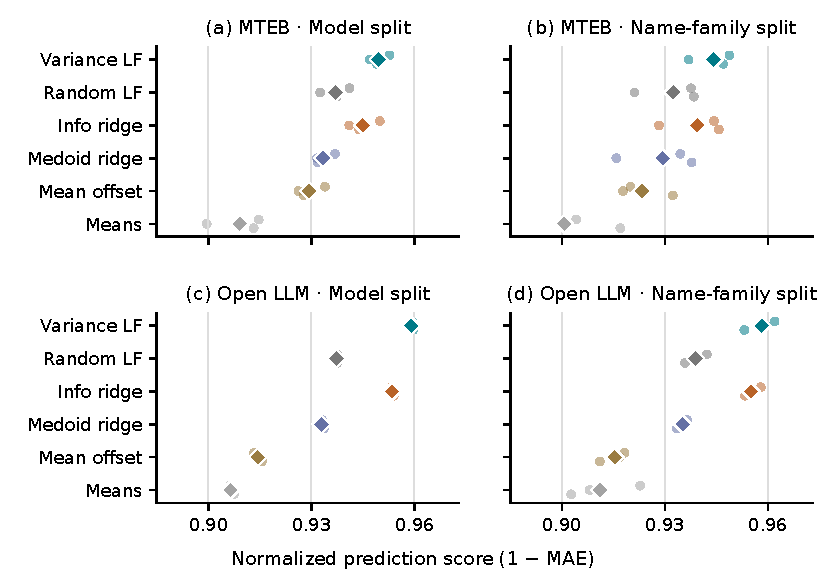
\includegraphics[width=\textwidth]{figures/main_comparison.pdf}
\caption{Direct comparisons under (a) MTEB model separation, (b) MTEB name-family separation, (c) Open LLM model separation, and (d) Open LLM name-family separation. Small dots show the three final seeds; diamonds show their means. Horizontal positions share the same explicitly restricted score axis. No dots are uncertainty intervals. Variance LF has the highest mean in each panel; the individual-seed reversal against Info ridge remains visible in panel (d).}
\label{fig:main}
% @evidence[[paper_data.json#final_evaluation.evaluation_evidence.episodes]]
\end{figure}

\subsection{Source, split, and seed heterogeneity}
Figure~\ref{fig:main} retains all source/split conditions instead of displaying only the pooled ranking. Mean Variance LF scores are $0.9496$ and $0.9442$ on MTEB's model and name-family splits, and $0.9591$ and $0.9582$ on Open LLM's corresponding splits. The pooled source scores are $0.9469$ for MTEB and $0.9586$ for Open LLM. These are not controlled source-difficulty comparisons: the benchmark collections, availability patterns, and budget ranges differ.
% @evidence[[derived_results.json#conditions]]
% @evidence[[paper_data.json#final_evaluation.metrics.mteb_score]]
% @evidence[[paper_data.json#final_evaluation.metrics.open_llm_score]]

The matched random-query factor baseline has lower observed scores in every retained source/split/seed cell. However, universal dominance across all comparators is not observed. On Open LLM's name-family split at seed $1019$, Variance LF scores $0.953104$, whereas Info ridge scores $0.953316$. Rounding these to fewer digits can hide the reversal. This small counterexample is important because the pooled ordering alone could suggest that the factor representation is always preferable. The evidence supports neither that conclusion nor isolated attribution to factorization rather than query selection.
% @evidence[[paper_data.json#final_evaluation.evaluation_evidence.episodes]]

The supplementary checkpoint curves show increasing observed scores with larger budgets along each retained trajectory. They cannot determine a universally sufficient $k$: there is no externally specified acceptable error threshold, no uncertainty interval by budget, and fewer available targets remain at later checkpoints. Nor do the summaries contain baseline checkpoint curves from which to infer budget-specific advantages over ridge. The central comparison is the prespecified average over checkpoint budgets.
% @evidence[[paper_data.json#final_evaluation.evaluation_evidence.episodes]]

\subsection{Sensitivity to historical correspondence}
Figure~\ref{fig:control} pairs the actual and deranged-history measurements. The pooled studied score falls from $0.9528$ to $0.9234$, an actual-minus-control gap of $0.02937$. Every retained source/split/seed pair has a lower observed score under the control. Useful historical structure therefore survives the source extraction and splitting procedures sufficiently to affect the measured policy. Benchmark marginals alone are not enough to reproduce its actual-history result.
% @evidence[[paper_data.json#final_evaluation.metrics.corruption_gap]]
% @evidence[[paper_data.json#final_evaluation.metrics.permuted_score]]
% @evidence[[paper_data.json#final_evaluation.evaluation_evidence.episodes]]

\begin{figure}[t]
\centering
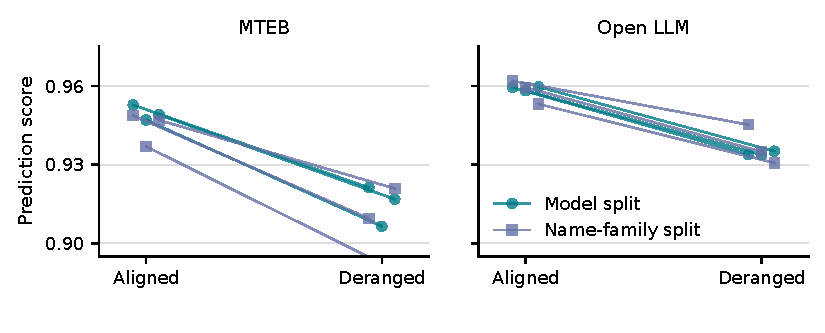
\includegraphics[width=\textwidth]{figures/historical_dependence_control.pdf}
\caption{Historical-correspondence control by source. Each line joins aligned and independently column-deranged histories for one retained seed and split; it does not depict temporal change. Color and marker distinguish split definitions. The control changes the learned representation and potentially the query set, so the score gap is not an acquisition-only effect.}
\label{fig:control}
\end{figure}

This is a dependence check, not proof that the low-rank model is true. The control perturbs factor learning, selection, and prediction jointly, and could also alter which targets remain. It cannot identify the best latent rank, verify that missingness is ignorable, or certify absence of benchmark contamination. All required final cases completed, and the reset replay passed; these facts support execution consistency within the tested interface, not comprehensive scientific validity.
% @evidence[[paper_data.json#final_evaluation.metrics.failed_episode_fraction]]
% @evidence[[paper_data.json#final_evaluation.metrics.reset_replay_ok]]

\section{Discussion and Limitations}
\paragraph{What the comparison identifies.}
The evidence is strongest for a policy-level statement: for these public score matrices, splits, and checkpoint weights, variance-guided factor reconstruction improves the observed remaining-target objective over its random-query counterpart. This is a useful decision problem when the evaluator cares precisely about whichever available benchmarks were not purchased. It is a weaker basis for a statement about reconstructing a prespecified panel, because the policy controls the scored target composition as well as the information collected. A fixed untouched panel, shared query sets for predictor ablations, and a selector-only comparison on that panel would separate these effects; none is reported here.

\paragraph{What the mechanism does not establish.}
The acquisition formula uses a conditional quadratic proxy with a unit-noise working interpretation. No empirical calibration of that uncertainty is available. The optimized proxy includes a coordinate that subsequently leaves the target set, and the final score uses absolute rather than squared loss. These mismatches do not invalidate the observed contrast, but they prevent interpreting it as validation of an optimality theorem. Likewise, availability-conditioned sequential choices should not be described as learning which question to ask from a new model's answers: the implemented choice ignores those answers.

\paragraph{Scope of the data distribution.}
Historical scores are selectively observed. Coverage filtering and the supplied availability mask restrict the population to models with enough measured benchmarks, potentially excluding the hardest prospective cases. Name-derived family labels can miss cross-namespace relationships and do not guarantee separation of pretraining data, fine-tuning lineages, or shared evaluation contamination. Historical-cell rank selection also does not measure sensitivity to tuning on entirely unseen families. The final splits and derangement control constrain some interpretations, but they do not justify arbitrary out-of-distribution or future-model generalization. Implementation interpretation uses the inspectable retained source; an independently verifiable byte-identical final snapshot is unavailable, as detailed in the supplement.

\paragraph{Uncertainty, costs, and practical use.}
The supplied bootstrap interval concerns one pooled matched-factor contrast under heuristic family clustering. It is not evidence of significance against all baselines; subgroup differences and the ridge comparison remain descriptive. The experiment purchases benchmark scores retrospectively from a frozen table and assumes equal query costs. It therefore demonstrates prediction under a score budget, not measured savings in inference time, energy, or monetary cost. A practical evaluator should select its own error tolerance, retain direct measurement of safety-critical or poorly represented benchmarks, and test a fixed target panel before relying on inferred scores for model release decisions.

\paragraph{What averaging hides.}
Equal row weights give sparse and dense held-out models the same contribution after their target errors are averaged. Equal source weights likewise prevent the larger generative-model table from overwhelming the embedding-model setting. These are explicit priorities of the evaluation, not invariances of the underlying inference problem. A different deployment population, benchmark weighting, or cost model can change the policy ranking. Moreover, a small average absolute error can coexist with large errors on a particular capability. The retained summaries contain neither per-benchmark residual distributions nor tail-error intervals, so they do not support certifying individual benchmark predictions, identifying which tasks can safely be skipped, or converting the pooled score into a deployment-specific reliability threshold. Reporting the source/split views and the local ridge reversal is therefore necessary, but not a substitute for task-level validation when choosing an actual evaluation panel.

\section{Conclusion}
Historical leaderboard measurements can support budgeted reconstruction without fitting a large predictor or running new language-model inference. In the evaluated setting, a regularized masked factor model coupled to variance-guided queries yields a higher pooled remaining-target score than the same factor construction with random queries. The historical-column control further shows that useful correspondence across benchmarks contributes to the measured result. These observations hold across the separately fitted embedding-model and generative-model sources and their two split definitions, rather than establishing transfer of a common representation.

The most important qualification is the target itself. Query policies remove different coordinates from evaluation, and the strongest covariance comparator is competitive, including a retained local reversal. The measurements therefore do not establish fixed-target superiority, score-adaptive selection, calibrated uncertainty, or a universal number of sufficient benchmarks. The appropriate conclusion is narrower: variance-guided masked reconstruction is a useful operational policy in the observed regime, with clear reasons to require shared-target evaluation, stronger family definitions, and explicit deployment costs before making broader claims.

\clearpage
\bibliography{references}
\bibliographystyle{paper}

\clearpage
\appendix
\section{Supplementary Information}
\subsection{Inspectable implementation and analytic identity}
The retained evaluated implementation is supplied at
\path{source_evidence/downstream/program/src/program.py}; the original reference is at
\path{source_evidence/downstream/baseline/src/program.py}.
Their readable source contents match. The entrypoint contract is in the adjacent \texttt{program\_spec.toml} files. Factor fitting is at lines 45--62, rank selection at lines 65--83, acquisition at lines 114--127, and conditional prediction at lines 134--142. Comparison implementations are inspectable in \path{source_evidence/evaluation/evaluate_final.py}, especially \texttt{reference\_fit}, \texttt{run\_baseline}, and \texttt{curve\_score}. These files, rather than source hashes alone, support the implementation description. The final manifest and the selection registry record different tree digests; no separate final source snapshot is supplied. We therefore do not certify byte-level identity of the final snapshot from hashes or method-family alignment alone. Implementation-level interpretation is conditional on the supplied retained-source association; final measurements and qualification are read independently from evaluator evidence.
% @evidence[[source_evidence/downstream/program/src/program.py]]
% @evidence[[source_evidence/downstream/baseline/src/program.py]]
% @evidence[[source_evidence/evaluation/evaluate_final.py]]

For completeness, set $H_Q=V_Q^\top V_Q+\lambda I$. Since $\lambda>0$, $H_Q$ is invertible. Multiplying $H_Q+v_av_a^\top$ by the right side of Equation~\ref{eq:rankone} gives the identity matrix: the added rank-one terms cancel after division by $1+v_a^\top C_Qv_a$. Multiplying the covariance difference on the left by $V_T$ and on the right by $V_T^\top$ and taking a trace gives
\[
 \operatorname{tr}\!\left[V_T(C_Q-C_{Q\cup\{a\}})V_T^\top\right]
 =\frac{\|V_TC_Qv_a\|_2^2}{1+v_a^\top C_Qv_a}.
\]
This matches the source acquisition calculation. It assumes the same target matrix on both sides and therefore is not a derivation of the actual change in remaining-target MAE. The factor estimates and regularization are treated as fixed; uncertainty about the fitted factors is not integrated out as in a fully Bayesian factor model.
% @evidence[[source_evidence/downstream/program/src/program.py#L114-L127]]

\subsection{Pinned acquisition, extraction, and reproducibility}
The MTEB score archive is pinned to revision
\texttt{6dabbcc68c28ea5f180c\allowbreak e7df79347b3ca9cc6383}
of \url{https://github.com/embeddings-benchmark/results}.
The Open LLM contents table is pinned to
\texttt{9c09a7cae43334062a82\allowbreak cb164f2ef255013dafa2}
at \url{https://huggingface.co/datasets/open-llm-leaderboard/contents}.
The acquisition audit, extracted private research pool, and final protocol are supplied in \path{source_evidence/evaluation/audit.json}, \path{task/resources/final/pool.json.gz}, and \path{source_evidence/evaluation/plan.json}. Reacquisition should verify the archive/table hashes recorded in the audit and reapply the documented extraction rather than substitute a current leaderboard. The audit attributes CC0-1.0 to the MTEB results according to the task data specification; it also notes the absence of a standalone license file in the pinned archive. The Open LLM dataset license is undeclared. Public access is not permission to redistribute that table; reproduction should reacquire it rather than assume redistribution rights.
% @evidence[[source_evidence/evaluation/audit.json#sources,extraction]]

Repeated MTEB model/column measurements use the deterministic lexicographically first revision. Exact duplicate raw documents retain only the archive-first owner and other copies become missing before splitting. Full score-example hashes are computed before downstream preprocessing. The family heuristic combines namespace and a lowercased model stem before punctuation/digits; Open LLM uses the base-model metadata when available. Such deterministic bookkeeping is reproducible but cannot recover unrecorded lineage.

The documented evaluation environment is CPython 3.12.15 on Linux x86\_64, NumPy 1.26.4, SciPy 1.12.0, and PyArrow 16.1.0. The benchmark evaluator requires native Landlock and seccomp isolation and a broker; a portable invocation on an unsupported kernel is not an equivalent reproduction. The exact entrypoint command is
\begin{samepage}
\begin{verbatim}
python task/evaluate_final.py \
  --program_path \
  source_evidence/downstream/program/src/program.py \
  --results_dir /tmp/reproduced-final
\end{verbatim}
\end{samepage}
The command is documented for independent reproduction on a supported isolated host, not rerun during manuscript preparation; production used the broker-mediated interface. Seeds are fixed by the evaluator to $1009,1013,1019$. The retained seed records report approximately $24.08$, $22.89$, and $23.08$ seconds respectively, excluding independent source acquisition. These are machine-dependent durations, not a runtime guarantee. No end-to-end acquisition/storage or benchmark-inference runtime was measured for this paper.
% @evidence[[source_evidence/evaluation/plan.json#runtime]]
% @evidence[[source_evidence/evaluation/requirements.txt]]
% @evidence[[paper_data.json#final_evaluation.evaluation_evidence.episodes]]

All manuscript tables and quantitative figures are generated by \path{build_paper_artifacts.py} directly from \path{paper_data.json}; this only summarizes saved measurements. The conceptual overview is prepared separately from the manuscript specification. \path{README.md} gives figure/table mappings and build commands. Derived artifacts have adjacent provenance sidecars and the manuscript has inline evidence links in LaTeX comments.

\subsection{Complete retained seed comparisons}
Table~\ref{tab:seeds} gives each primary source/split/seed comparison. The pooled weighting averages target errors within rows before averaging rows and checkpoints, then gives equal weight to seeds, the two split cases per source, and the two sources. The reset replay is omitted here and from primary aggregates. Table~\ref{tab:controls} retains all actual/control pairs for the studied policy; control scores are not mixed into the primary leaderboard.

\begin{table}[h]
\centering\footnotesize
% @evidence[[paper_data.json#final_evaluation.evaluation_evidence.episodes]]
\begin{tabular}{llrrrrrr}\toprule Source & Split/seed & Var LF & Rand LF & Info R & Med R & Offset & Means \\ \midrule
MTEB & M/1009 & 0.9528 & 0.9412 & 0.9500 & 0.9369 & 0.9340 & 0.9147 \\
MTEB & M/1013 & 0.9470 & 0.9326 & 0.9410 & 0.9316 & 0.9262 & 0.8996 \\
MTEB & M/1019 & 0.9490 & 0.9373 & 0.9439 & 0.9318 & 0.9277 & 0.9132 \\
\addlinespace
MTEB & F/1009 & 0.9488 & 0.9376 & 0.9443 & 0.9345 & 0.9199 & 0.9042 \\
MTEB & F/1013 & 0.9369 & 0.9211 & 0.9283 & 0.9158 & 0.9178 & 0.8810 \\
MTEB & F/1019 & 0.9469 & 0.9384 & 0.9457 & 0.9378 & 0.9323 & 0.9170 \\
\addlinespace
Open LLM & M/1009 & 0.9595 & 0.9375 & 0.9535 & 0.9331 & 0.9133 & 0.9063 \\
Open LLM & M/1013 & 0.9582 & 0.9370 & 0.9529 & 0.9321 & 0.9143 & 0.9055 \\
Open LLM & M/1019 & 0.9597 & 0.9376 & 0.9540 & 0.9336 & 0.9156 & 0.9075 \\
\addlinespace
Open LLM & F/1009 & 0.9619 & 0.9422 & 0.9579 & 0.9364 & 0.9182 & 0.9228 \\
Open LLM & F/1013 & 0.9594 & 0.9387 & 0.9539 & 0.9359 & 0.9168 & 0.9081 \\
Open LLM & F/1019 & 0.9531 & 0.9358 & 0.9533 & 0.9334 & 0.9111 & 0.9027 \\
\addlinespace
\bottomrule\end{tabular}
\caption{All retained primary scores. M/F denotes model/name-family split; LF denotes low-rank reconstruction; R denotes ridge. Values are averages over the source-specific budget checkpoints, not single-budget scores.}
\label{tab:seeds}
\end{table}

\begin{table}[h]
\centering\small
% @evidence[[paper_data.json#final_evaluation.evaluation_evidence.episodes]]
\begin{tabular}{llrr}\toprule Source & Split/seed & Aligned & Deranged \\ \midrule
MTEB & M/1009 & 0.9528 & 0.9212 \\
MTEB & M/1013 & 0.9470 & 0.9065 \\
MTEB & M/1019 & 0.9490 & 0.9168 \\
MTEB & F/1009 & 0.9488 & 0.9094 \\
MTEB & F/1013 & 0.9369 & 0.8923 \\
MTEB & F/1019 & 0.9469 & 0.9209 \\
Open LLM & M/1009 & 0.9595 & 0.9338 \\
Open LLM & M/1013 & 0.9582 & 0.9338 \\
Open LLM & M/1019 & 0.9597 & 0.9351 \\
Open LLM & F/1009 & 0.9619 & 0.9452 \\
Open LLM & F/1013 & 0.9594 & 0.9349 \\
Open LLM & F/1019 & 0.9531 & 0.9307 \\
\bottomrule\end{tabular}
\caption{Historical-correspondence control for Variance LF. Each row is a paired source/split/seed comparison. M/F follows Table~\ref{tab:seeds}.}
\label{tab:controls}
\end{table}

\subsection{Budget-conditioned measurements}
Figure~\ref{fig:budget} displays only the measured studied-policy checkpoint curves. The retained records provide comparison-policy averages but not their checkpoint arrays. Consequently, this figure makes no budget-specific comparative claim. Later checkpoints remove more benchmarks from the target set, which is another reason not to read the curves as a fixed-panel learning curve or as evidence that a particular budget is sufficient.

\begin{figure}[h]
\centering
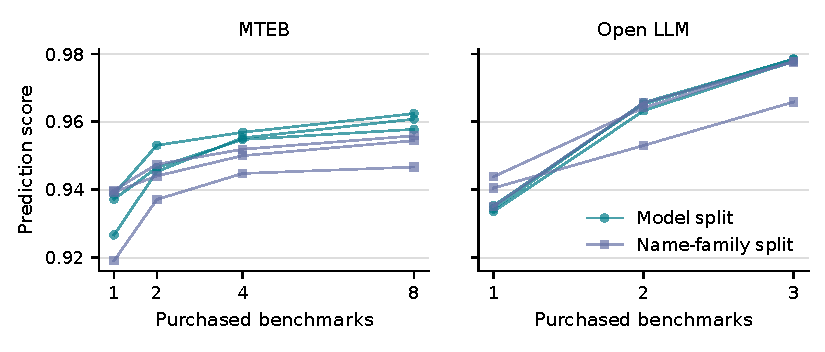
\includegraphics[width=\textwidth]{figures/budget_sensitivity.pdf}
\caption{Recorded checkpoint scores for Variance LF. Each line is one split and seed; all measured trajectories are shown. The Open LLM and MTEB budget grids differ. These are budget-conditioned remaining-target scores, not measurements of comparison policies or a fixed evaluation panel.}
\label{fig:budget}
% @evidence[[paper_data.json#final_evaluation.evaluation_evidence.episodes]]
\end{figure}

\subsection{Uncertainty and evaluation provenance}
The supplied bootstrap uses evaluator RNG seed $24681357$. Family multiplicities are drawn per source and shared over paired Variance LF/Random LF observations, cases, and seeds. Equal case, seed, and source weights are preserved. Zero sampled mass for a case/seed contributes zero rather than changing its aggregation weight; incomplete required actual measurements would trigger a conservative interval. These are the documented resampling semantics, not a new analysis from unavailable row residuals. The family labels are heuristic, so the interval is conditional on that clustering choice.
% @evidence[[source_evidence/evaluation/plan.json#uncertainty]]

The final evidence independently records completion and qualification. This is distinct from retaining the original reference after a selection procedure with zero measured score change and three unscored alternative evaluations. Missing scores are missing performance evidence, not measured losses. Their recorded exits do not identify statistical failure, protocol invalidity, or adaptivity defects as the cause. No alternative-method performance table, successful nonlinear comparison, fixed-target ablation, or family-held-out hyperparameter tuning is inferred from these records. Candidate-generated diagnostic descriptions were not trusted as verified measurements.
% @evidence[[paper_data.json#downstream_study]]
% @evidence[[paper_data.json#final_evaluation.evaluation_evidence.candidate_diagnostics_trust]]
% @evidence[[paper_data.json#final_evaluation.outcome]]

\subsection{Research transparency}
This observational study analyzes public model-level scores and does not collect new human-subject data. The main risks are misleading inferred model capabilities and overconfident deployment decisions, especially under selective missingness or lineage shift. Inferred scores should not replace direct evaluation of high-stakes properties. No claim of a universal ranking, proprietary-data access, or a measured environmental benefit is made. Negative and countervailing observations, including the local ridge reversal and lack of scored alternative-method evidence, are retained.

Literature access was restricted to explicitly permitted starter records and exact foundational-method identifiers/titles. No citation graph expansion or broad search for the prohibited related work was performed. Retrieved metadata and abstracts were checked for relevance; mismatched records and an unrelated abstract were rejected rather than cited. The active citation provenance records the content actually consulted. No prohibited-material encounter was identified during this writing step.

\subsection{LLM Usage}
LLM-based agents assisted with research proposals, source implementation, framing, literature-metadata checking, and manuscript preparation. The exploratory alternative implementations did not yield usable comparative scores; the evaluated method remained the supplied reference. For this manuscript, an LLM inspected saved source and evaluator evidence, selected the bounded empirical thesis, generated static plotting/table code, drafted and revised the text, and ran grounding and LaTeX checks. It did not rerun the final experiments or create new performance measurements. Literature claims were limited to consulted allowed abstracts and the explicitly retrieved factorization paper. No human review, human-conducted experiment, or independent external replication is implied.

\end{document}
